\documentclass[11pt]{report} %size of font and type of layout
\usepackage[twoside,a4paper,margin=1in]{geometry} %change margin size for binding later?
\usepackage[T1]{fontenc}
\usepackage[bitstream-charter]{mathdesign} % another font option

%\usepackage{kpfonts}%  for math    
%\usepackage{libertine}%  serif and sans serif default writing
%\usepackage[scaled=0.85]{beramono}%% mono for typewriter font

%\usepackage{pgfplots}
%\usepackage{tikz}
\usepackage{xfrac}
\usepackage[super]{nth} %allow 1st, 2nd by typing \nth{1}, \nth{2}
\usepackage[toc,title,titletoc,page]{appendix} %for using appendices
\usepackage{graphicx} %have images
\usepackage{chngcntr} %be able to make figures go 1, 2, 3 instead of 1.1, 1.2, 1.3, etc
\usepackage{subcaption} %have subfigures
%\usepackage{wrapfig} %be able to wrap text around figures
%\usepackage{amsmath} %a way to typeset maths
%\usepackage{amssymb} %able to type maths symbols
\usepackage{textcomp} %so we can use \textdegree to get degree symbol
\usepackage[parfill]{parskip} %remove paragraph indentation
\usepackage{setspace} %be able to set line spacing
\usepackage{tocloft} %more control over table of contents, list of figures, etc
\usepackage{ltxtable} %get tabularx split over pages
\usepackage[english]{babel} %english-specific charaters and language rules
\usepackage{url} %type urls
\usepackage{parskip} %space between paragraphs
\usepackage[UKenglish]{isodate} %change date format
%\usepackage[hang,flushmargin]{footmisc} %no indents in footers
%\usepackage{verbatimbox} %able to use addvbuffer to change spaces before and after tables
\usepackage{pdfpages} %insert PDF pages
%\usepackage{titletoc} %create a small table of contents at the start of each section
\usepackage{microtype} %improves spacing between words and letters
\let\ordinal\relax
\usepackage[nodayofweek]{datetime} %use \today to get the date
\usepackage[inline]{enumitem} %have inline lists
\usepackage{fancyhdr}		%for getting customized headers
%\usepackage{lastpage}		%enable getting the total of the pages
%\usepackage{floatrow} %use for indicating figures' sources
%\usepackage{showframe} %show margins on page
\usepackage[hidelinks]{hyperref} %hyperlinks in pdf
\usepackage{cleveref} %automatic referencing
\usepackage{bookmark}
\DeclareGraphicsExtensions{.pdf,.png,.jpg,.eps} %can just give images' names
\usepackage{epstopdf} %allows for encapsulated postscript vector images, better quality and scalable
\usepackage[none]{hyphenat}		%kills all word breaks that were in annoying places
\usepackage{lipsum}

%--------------------------heading spacings----------------------------%
\usepackage{titlesec} %be able to change title settings
	\titleformat{\chapter}{\normalfont\huge\bfseries}{\thechapter.}{1em}{} %have number before chapter title
	\titlespacing{\chapter}{0pc}{0pc}{0pc} %have nice spacing after chapter title {indent} {before} {after}
	\titlespacing{\section}{0pc}{1pc}{0pc} %have nice spacing after section title {indent} {before} {after}
	\titlespacing{\subsection}{1pc}{1pc}{0pc} %have nice spacing after subsection title {indent} {before} {after}
	\titlespacing{\subsubsection}{0pc}{0pc}{-1pc} %have nice spacing after subsection title {indent} {before} {after}
	\titlelabel{\thetitle.\quad} %full stop after the number in the heading title
\usepackage{etoolbox} %remove page break before chapter heading
	\makeatletter
	%\patchcmd{\chapter}{\thispagestyle{plain}}{}{}{} %allows the header/footer on chapter pages
	\patchcmd{\chapter}{\if@openright\cleardoublepage\else\clearpage\fi}{}{}{}
	\makeatletter
	%\newcommand{\updatechaptermark}{%
	\appto\ps@fancy{%
		\patchcmd{\chaptermark}% <cmd>
		{\@chapapp\ }{}% <search><replace>
		{}{}% <success><failure>
	}%}
	\makeatother
%----------------------------figures & lof (list of figures)-----------------------------%
\renewcommand{\cftfigfont}{Figure } %list of figures includes "Figure"
\newcommand*{\noaddvspace}{\renewcommand*{\addvspace}[1]{}}\addtocontents{lof}{\protect\noaddvspace} %equal line spacing in the list of figures
\setlength{\cftfigindent}{0pt} %remove indentation from figures in lof
\usepackage{float} %able to use H to force figures to go here
%\floatstyle{boxed}	%this will place a thin border around my figures
%\restylefloat{figure}
\AtBeginEnvironment{figure}{\vspace{10pt}} %spacing before figure
\AtEndEnvironment{figure}{\vspace{-10pt}} %spacing after figure
\setlength{\abovecaptionskip}{10pt} %spacing before figure caption
\setlength{\belowcaptionskip}{5pt} %spacing after figure caption
\usepackage[justification=centering,font={normalsize, it}]{caption} %control caption text
%----------------------------tables & lot------------------------------%
\renewcommand{\cfttabfont}{Table } %list of tables includes "Table"
\setlength{\cfttabindent}{0pt} %remove indentation from tables in lot
\usepackage{tabularx} %word wrap in tables
\usepackage{longtable} %allow tables to go over multiple pages
\usepackage{multirow} %make cells span multiple rows in tables
\captionsetup{belowskip=5pt,aboveskip=4pt}
\newcolumntype{L}{>{\centering\arraybackslash}m{3cm}} %centre and wrap text in tables
\usepackage{booktabs} %use \toprule, \midrule, \bottomrule and \cmidrule for better spacing in tables
\usepackage{pbox} %force line break in a table cell
%---------------------------create own lists---------------------------%
\newlistof{example}{exp}{List of Examples} %create own lists
\newcommand{\example}[1]{ %create own lists
	\refstepcounter{example} %create own lists
	\par\noindent\textbf{Example \theexample. #1} %create own lists
	\addcontentsline{exp}{example} %create own lists
	{\protect\numberline{\thechapter.\theexample}#1}\par} %create own lists
%---------------------------------font---------------------------------%
%\sfdefault = calibri-like font, \rmdefault = times new roman-like
%\renewcommand\UrlFont{\rmfamily}
%\renewcommand{\familydefault}{\rmdefault}
%----------------------------------------------------------------------%
\begin{document}
\begin{onehalfspace} %single line spacing
%\counterwithout{figure}{chapter} %makes figures go 1, 2, 3 instead of 1.1, 1.2, 1.3, etc
%\counterwithout{table}{chapter} %makes tables go 1, 2, 3 instead of 1.1, 1.2, 1.3, etc
%\counterwithout{section}{chapter} %make sections 1, 2, 3 not 1.1 etc
\pretolerance=10000 %disable hyphenating at line breaks
\abovedisplayskip=5pt %remove space before equations
\belowdisplayskip=5pt %remove space after equations
\cleanlookdateon %remove current date format to replace with [UKenglish]{isodate}
%\let\savenumberline\numberline\def\numberline#1{\savenumberline{#1.}} %adds dot after chapter title in toc, comment this out to get appendices to work and not cause spacing errors.
%\AtEndEnvironment{itemize}{\vspace{-5pt}} %spacing after lists

\newcommand{\thetitle}	{Jump stabilization using a \\ spider-like drag line}
\newcommand{\theauthor}	{Roberto Aldera}
\newcommand{\studentnum}{ALDROB001}
\newcommand{\thedate}	{\today}
\newcommand{\coursecode}{EEE4022S}
\newcommand{\coursename}{Course Name}
\newcommand{\staffmember}{Dr. Amir Patel}

\pagenumbering{gobble}	%no page number for title page
\renewcommand\headrulewidth{0pt}	%get rid of stray header underline
\begin{minipage}{1\textwidth}
\begin{center}
\Huge\textbf{\thetitle}
\vskip20pt
%\hrule
\vskip50pt

\includegraphics[width=0.45\linewidth]{UCTcircular}
\vskip50pt
\vskip20pt
\Large{\textbf{\theauthor\\
\Large\studentnum\\
\nth{4} year BSc. (Eng) Mechatronics\\
\vskip70pt
\coursecode \\
Supervisor: \staffmember \\
Department of Electrical Engineering\\
University of Cape Town \\
\vskip20pt
\thedate}}\\
\end{center}
\end{minipage}
\newpage 
\clearpage\mbox{}\clearpage

\pagenumbering{roman}	%start the page numbering (and reset it to zero)
\cleardoublepage
\phantomsection

\addcontentsline{toc}{chapter}{Declaration}	
\chapter*{Declaration}
I know that plagiarism is wrong. Plagiarism is to use another's work and pretend that it is my own.

I have used the IEEE convention for citation and referencing. In this thesis, all contributions to, and quotations from, the work(s) of other people have been cited and referenced. 

This thesis is my own work. I have not allowed, and will not allow, anyone to copy my work.
\vskip100pt
\begin{center}
	Signed: \line(1,0){200}
	\vskip20pt
	Dated: \line(1,0){200}
\end{center}

\newpage

\addcontentsline{toc}{chapter}{Abstract}
%Thesis abstract here.
\chapter*{Abstract}
This thesis investigates aerial stabilisation of a bio-inspired jumping robot using a spider-like dragline. Previous work on pitch angle control by Shield \cite{StaceyThesis} (and others too) is expanded upon to include a mechanical leg for jumping as well as controller design for precision jumping. By using a position estimator, the platform's position can be established and treated as a control problem. A discussion on the use of the spider's dragline for precision jumping is presented and provides the basis for the problem formulation. 

Add additional things here once results are known.
\newpage
\phantomsection

\addcontentsline{toc}{chapter}{Acknowledgements}	
%Thesis acknowledgements
\chapter*{Acknowledgements}
Acknowledge people here...
\newpage
\phantomsection

\addcontentsline{toc}{chapter}{Table of Contents}
\renewcommand{\contentsname}{Table of Contents} %change table of contents's name from 'contents' to 'table of contents'
\newpage %page break
\phantomsection %for some reason this gets the bookmarks to work

\tableofcontents



%\addcontentsline{toc}{chapter}{Section:} %add "table of contents" to the table of contents
\newpage %page break
\newpage
\phantomsection

\addcontentsline{toc}{chapter}{List of Figures}
\listoffigures
\newpage
\phantomsection

\addcontentsline{toc}{chapter}{List of Tables}
\listoftables
\newpage

\renewcommand\headrulewidth{0.5pt}
\pagenumbering{arabic}	%start the page numbering (and reset it to zero)

\pagestyle{fancy}
\fancyhf{}
%\chead{\leftmark}
\cfoot{\thepage}
\fancyhead[LE]{\textit{\leftmark}}
\fancyhead[RO]{\textit{\leftmark}}
\setlength{\headheight}{14pt} 

%Introduction
\chapter{Introduction}
\section{Background}
\lipsum[1]
\section{Research Objectives}
\lipsum[1]
\section{Scope and Limitations}
\lipsum[1]
\section{Plan of Development}
\lipsum[1-9]
\pagebreak
%Literature review
\chapter{Literature Review}
\section{Introduction}
\lipsum[1]
\section{Another few sections}
\lipsum[1]
\section{Summary and Conclusions}
\lipsum[1]

Review some literature here \cite{StaceyThesis}.
\begin{figure}
	\centering
	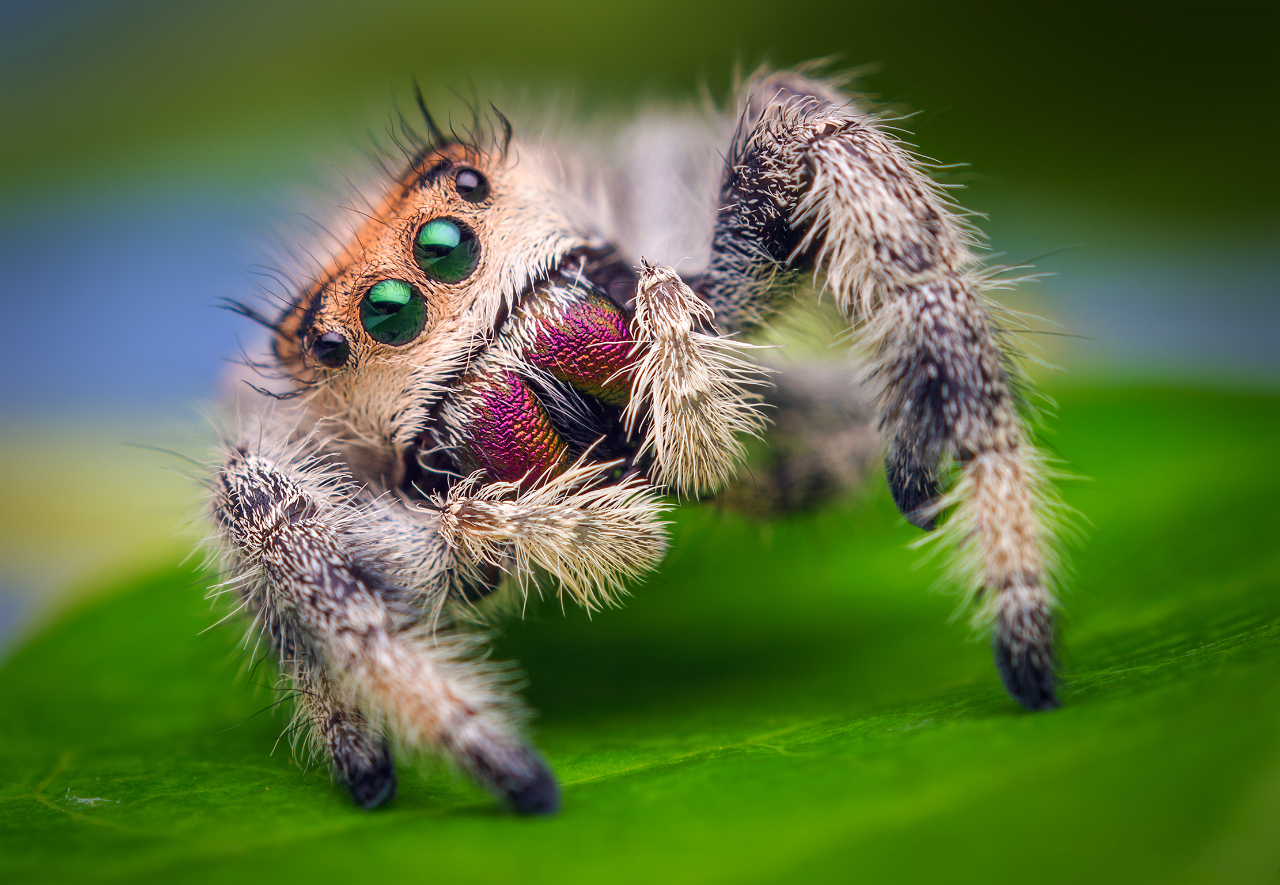
\includegraphics[width=0.7\textwidth]{images/spidey}
	\vskip10pt
	\caption[The caption that appears in the list of figures]{The caption that appears under the figure}
	\label{fig:exam}
\end{figure}
\lipsum[1-5]
\pagebreak
%Literature review
\chapter{Theory Development}

Develop some theory and solve for $x$ afterwards.

$$\int_{0}^{\infty}x^2dx = \sum_{0}^{\infty} \theta \alpha \mu$$
Now for some \texttt{typewriter stuff for interest} just to test fonts.
\\
\lipsum[1-7]
\pagebreak
%Literature review
\chapter{Methodology}


\lipsum[1-20]
\pagebreak
%Literature review
\chapter{System Modelling and Simulation}


\lipsum[1-2]
\pagebreak

%Literature review
\chapter{Mechanical Design}

%TODO - Nautilus cam gear, platform inherently stable
Develop some theory.

\lipsum[1-10]
\pagebreak

%Literature review
\chapter{Controller Design}

Develop some theory.
\lipsum[1-20]
\pagebreak
%Literature review
\chapter{Model Verification}

Develop some theory.
\lipsum[1-20]
\pagebreak
%Literature review
\chapter{Testing and Implementation}

Develop some theory.
\lipsum[1-20]
\pagebreak
%Literature review
\chapter{Discussion}

Develop some theory.
\lipsum[1-20]
\pagebreak
%Literature review
\chapter{Conclusions and Recommendations}

Develop some theory  for Future Work
\lipsum[1-2]
\pagebreak


\newpage
\addcontentsline{toc}{chapter}{References}
\begingroup
\raggedright
\renewcommand\bibname{References}
\bibliography{Aldera_bibliography}
\bibliographystyle{ieeetran}
\endgroup
%\counterwithin{section}{chapter} %make sections 1.1, 1.2 etc again, this undoes counterwithout
\begin{appendices}
	%\renewcommand{\appendixtocname}{List of appendices}
	\renewcommand{\appendixname}{}% Change "chapter name" for Appendix chapters
	
	\appendix
	%\appendixpage
	%\addappheadtotoc
\chapter{Insert Here}
\label{app:Insert Here}	
\section{Craig}
\newpage

\chapter{Another}
\label{app:Another}
\end{appendices}	%for use with appendices
\newpage	%this keeps the header/footer working on the last page. Do not type anything after this.
\end{onehalfspace}
\end{document}

%-------------------------------Figures--------------------------------%
\begin{figure}[H]
\centering
\includegraphics[width=0.4\textwidth]{images/%}
\vskip10pt
\caption[The caption that appears in the list of figures]{The caption that appears under the figure}
\label{fig:exam}
\end{figure}

\begin{figure}[H]
\centering
\begin{subfigure}[t]{0.49\textwidth}
\centering
\includegraphics[width=0.9\linewidth]{images/%}
\caption{This is figure a}
\label{fig:figureA}
\end{subfigure}
\begin{subfigure}[t]{0.49\textwidth}
\centering
\includegraphics[width=0.9\linewidth]{images/%}
\caption{This is figure b}
\label{fig:figureB}
\end{subfigure}
\caption{Caption}
\end{figure}

\begin{wrapfigure}{r}{0.5\textwidth}
\begin{center}
\includegraphics[width=0.48\textwidth]{images/ %}
\end{center}
\caption{A gull}
\end{wrapfigure}

As can be seen in \cref{fig:exam}\\
%-------------------------------Headings-------------------------------%
\chapter{Chapter Title}
\label{ch:Chapter Title}

\section{Section Title}
\label{sec:Section Title}

\subsection{Subsection Title}
\label{subsec:Subsection Title}

\subsubsection{Subsubsection Title}
\label{bb:Subsubsection Title}
%-----------------------------Insert Pages-----------------------------%
\includepdf[pages={1}]{ %filename.pdf}
%--------------------------------Citing--------------------------------%
\footnote{\cite{aa}}
\cite{aa,bb}